% Graphic: Equivalencias ECC
\begin{figure}[H]
    \centering
    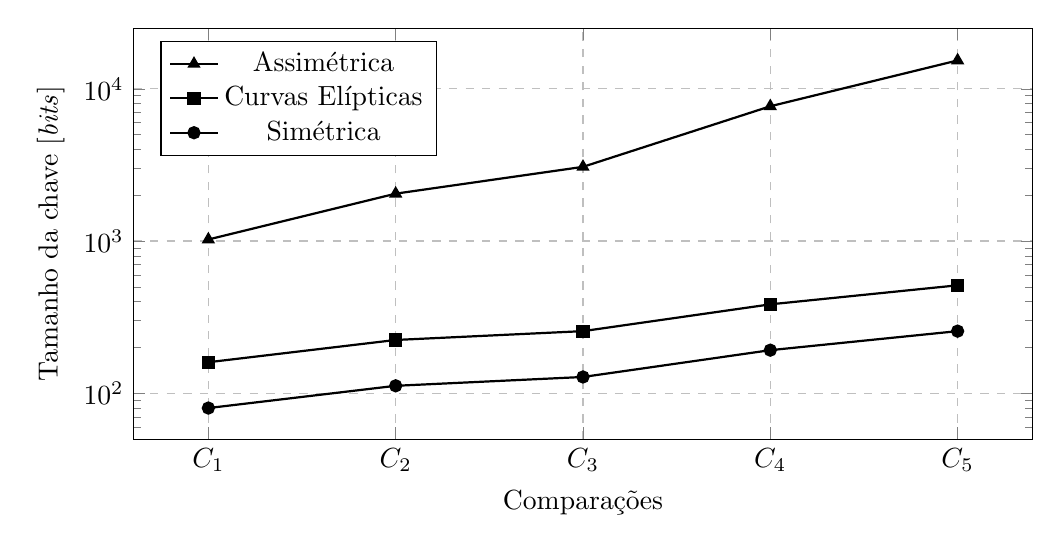
\begin{tikzpicture}
        \begin{semilogyaxis}[
            % title={Combinações possíveis para chaves binárias},
            ylabel={Tamanho da chave [\textit{bits}]},
            xlabel={Comparações},
            ymin=50, ymax=25000,
            symbolic x coords={$C_1$, $C_2$, $C_3$, $C_4$, $C_5$},
			xtick={$C_1$, $C_2$, $C_3$, $C_4$, $C_5$},
            legend pos=north west,
            ymajorgrids=true,
            xmajorgrids=true,
            grid style=dashed,
            height=6.8cm,
            width=13cm
        ]
			
		\addplot[color=black, solid, thick, mark=triangle*]
			coordinates {
				($C_1$,1024)
				($C_2$,2048)
				($C_3$,3072)
				($C_4$,7680)
				($C_5$,15360)
			};
			\addlegendentry{Assimétrica}
			
		\addplot[color=black, solid, thick, mark=square*]
			coordinates {
				($C_1$,160)
				($C_2$,224)
				($C_3$,256)
				($C_4$,384)
				($C_5$,512)
			};
			\addlegendentry{Curvas Elípticas}
			
		\addplot[color=black, solid, thick, mark=*]
			coordinates {
				($C_1$,80)
				($C_2$,112)
				($C_3$,128)
				($C_4$,192)
				($C_5$,256)
			};
			\addlegendentry{Simétrica}
     
        \end{semilogyaxis}
    \end{tikzpicture}
    \caption{Equivalência de chaves entre diferentes algoritmos criptográficos.}
    \label{graph:equivalencias_ecc}
\end{figure}
